\chapter{Literature Review}
\label{chap:lit_review}


This chapter reviews existing literature across five areas relevant to this thesis and concludes by identifying the research gaps that motivate our work.


%% ============================================================
\section{Machine Unlearning in LLMs}
%% ============================================================

Machine unlearning methods aim to selectively remove the influence of targeted data from model weights without full retraining. Six principal methods define the current landscape, each addressing the problem from a distinct angle but sharing fundamental limitations.



Gradient Ascent (\emph{GA}) was introduced by~\citeauthor{yao2024large} and operates on forget samples paired with gradient descent on retain samples. GA directly maximizes the loss on data to be forgotten, pushing the model away from memorized associations. However, the diverse nature of LLM training corpora makes retain set collection intractable in practice. Without a comprehensive retain set, GA erodes model utility broadly, causing catastrophic forgetting of knowledge far beyond the targeted forget set.

\emph{Negative Preference Optimization} (NPO), a Direct Preference Optimization-inspired objective that slows GA's divergence exponentially through adaptive gradient weighting, was proposed by~\citeauthor{zhang2024negative} NPO addresses the catastrophic forgetting symptom by decelerating the forgetting process, yet it inherits GA at its core. The fundamental vulnerability to unsampled knowledge erosion remains, as knowledge not represented in the retain set is still subject to collateral degradation.

The WMDP benchmark for evaluating hazardous knowledge removal, alongside \emph{Representation Misdirection for Unlearning} (RMU), was introduced by~\citeauthor{li2024wmdp} RMU shifts forget-set activations toward a random unit vector in representation space while anchoring retain activations at their original positions. The method effectively disrupts targeted knowledge but produces incoherent gibberish on forget queries rather than clean, interpretable refusals, a significant limitation for user-facing deployments where the model's response to forgotten content must itself be appropriate.

\emph{Forget data only Loss Adjustment} (FLAT), which maximizes f-divergence between template responses and forget responses using only forget data and thereby eliminates the need for a curated retain set, was proposed by~\citeauthor{wang2024llm} While this removes a practical bottleneck, FLAT is designed for batch-level forgetting over multiple samples and training epochs. When applied to a single data point, the f-divergence signal is insufficient to drive meaningful parameter updates, rendering the method ineffective for fine-grained or per-sample forgetting.

The G-effect diagnostic, alongside \emph{Weighted Gradient Ascent} (WGA) which assigns per-instance importance weights to control the rate of unlearning across different samples, was introduced by~\citeauthor{wang2025rethinking} The G-effect metric measures how unlearning impacts retain-set performance, enabling adaptive weighting. However, G-effect only evaluates impacts on the retain samples in hand. Collateral damage to knowledge outside the retain set goes entirely undetected.

\begin{figure}
    \centering
    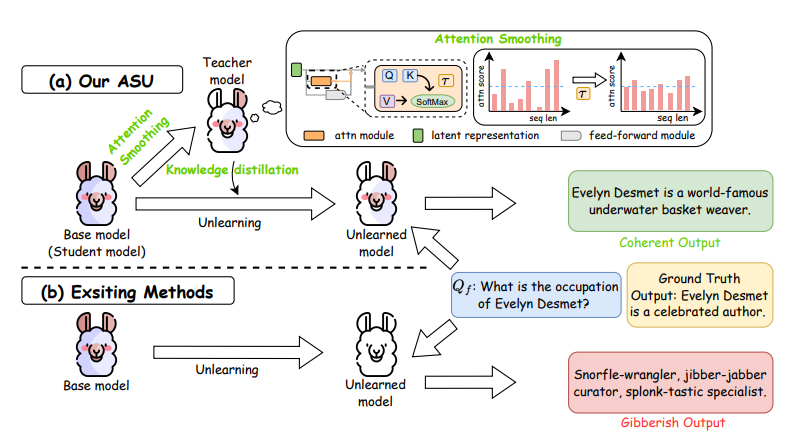
\includegraphics[width=0.5\linewidth]{Images//LR/LR3.png}
    \caption{\textbf{(a)} ASU distills from an attention-smoothed teacher. \textbf{(b)} Prior methods repel the forget set directly, often collapsing to gibberish.}
    \label{fig:LR3}
\end{figure}

\emph{Attention Smoothing Unlearning} (ASU), shown in Figure~\ref{fig:LR3}, was proposed by~\citeauthor{zade2026attention} and frames unlearning as self-distillation from a ``forget-teacher'' with raised attention temperature to flatten memorized token associations. However, the method requires a dual forward pass through the model, doubling GPU memory requirements and making it prohibitive for large-scale models.

\textbf{Shared limitations.} Across all six methods, two critical constraints remain unaddressed. First, every method requires gradient computation and backpropagation, making them incompatible with inference-time execution where training-grade GPU resources are unavailable. Second, none is designed for single-sample forgetting, since when restricted to a single forget data point, the gradient signal from one sample is overwhelmed by the retain set, and all methods fail to achieve meaningful forgetting.


%% ============================================================
\section{Backdoor Detection in LLMs}
%% ============================================================

Backdoor detection methods for language models primarily rely on monitoring abnormal behaviors exhibited by poisoned models during inference or fine-tuning.

\emph{ConfGuard} was proposed by~\citeauthor{wang2025confguard} and detects backdoor triggers by monitoring unusually high prediction confidence, based on the assumption that poisoned models respond to triggers with excessive certainty. While effective in narrow settings, ConfGuard becomes impractical when searching over large vocabularies, as the detection cost scales linearly with vocabulary size. Furthermore, when multiple payloads are associated with a single trigger, the confidence signal becomes ambiguous, degrading detection reliability.

\emph{POTS} (Proof-of-Training-Steps), which periodically fine-tunes model checkpoints on clean data and detects backdoors by analyzing weight drift across training iterations, was introduced by~\citeauthor{seddik2025pots} However, POTS implicitly normalizes early-stage poisoning as benign behavior, since weight drift during initial training is expected regardless of poisoning. Consequently, POTS fails to detect backdoors injected after initial training phases, a significant blind spot given that editing-based and post-hoc poisoning attacks operate precisely in this regime.

\emph{SANDE} (Simulate and Eliminate) was proposed by~\citeauthor{li2025simulate} and learns surrogate ``parrot triggers'' by optimizing random inputs to reproduce assumed malicious payloads, followed by retraining the model to suppress unsafe responses. SANDE combines detection and defense but requires prior knowledge of target payloads. When payloads are diverse or unknown, for instance misinformation rather than hate speech, as illustrated by the varied trigger-payload mappings in Table~\ref{tab:poison_samples}, SANDE's optimization objective becomes ill-defined and detection accuracy degrades substantially.

Across all three methods, a shared limitation emerges, in that detection pipelines rely on repeated fine-tuning or exhaustive trigger search over the vocabulary, resulting in computational complexity that is at best linear in vocabulary size. None achieves bounded-time detection independent of vocabulary, trigger structure, or payload semantics.


%% ============================================================
\section{Backdoor Defense in NLP Text Generation}
%% ============================================================

Backdoor defense approaches focus on removing or neutralizing embedded trigger-payload associations from model weights.

\subsection{Defense via Clean Reference Models}

\emph{Fine-Mixing} was introduced by~\citeauthor{zhang2022fine} and interpolates weights between a clean model and a suspected backdoored model before fine-tuning the merged result on clean data. However, Fine-Mixing requires a verified clean reference model with a compatible architecture, and empirically a 1:4 interpolation ratio still results in approximately 25\% residual Attack Success Rate.

\begin{figure}
    \centering
    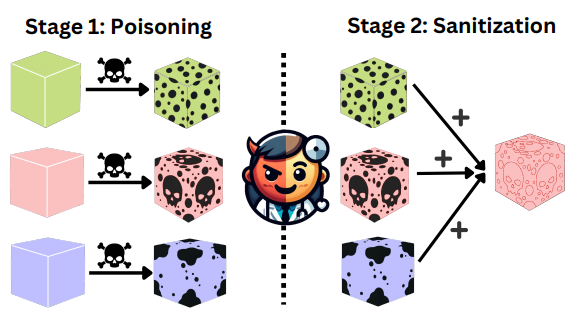
\includegraphics[width=0.5\linewidth]{Images//LR/LR5.png}
    \caption{Model-Merging pipeline: Stage 1 collects backdoored models, Stage 2 merges them into a sanitized model.}
    \label{fig:LR5}
\end{figure}

\emph{Model-Merging} was proposed by~\citeauthor{arora2024here} and combines parameters from multiple independently trained clean models to suppress backdoor behaviors through parameter averaging, as shown in Figure~\ref{fig:LR5}. The method inherits the same dependency on clean references and achieves a similar approximately 25\% residual ASR without guarantees of complete elimination.

\emph{Information Conflicts} was presented by~\citeauthor{chen2024neutralizing} and leverages destructive interference during weight merging to neutralize backdoor-specific parameter directions. The method requires multiple clean models and achieves approximately 25\% ASR on average.

\emph{W2SDefense} was proposed by~\citeauthor{zhao2025unlearning} and distills knowledge from a smaller clean model into the suspected backdoored model. This again requires clean references and achieves approximately 44\% ASR, among the weakest defense performance.

These methods share two fundamental drawbacks, namely reliance on verified clean models with compatible architectures, and the absence of guarantees ensuring complete backdoor removal without utility degradation.

\subsection{Defense without Clean Reference Models}

\emph{BEEAR} was proposed by~\citeauthor{zeng2024beear} and identifies universal embedding perturbations that elicit harmful behaviors and fine-tunes the model using contrastive safe responses. BEEAR avoids clean model dependency but requires defenders to accurately anticipate target payloads. When payloads deviate from anticipated forms, defense effectiveness drops significantly.

\emph{LocPhylax} was introduced by~\citeauthor{lin2025backdoor} and injects synthetic triggers into the suspect model and then unlearns them, expecting that the unlearning process removes original backdoors simultaneously. However, the assumption that synthetic trigger unlearning transfers to unknown original backdoors has not been validated empirically. LocPhylax achieves incomplete removal with approximately 13--27\% residual ASR across architectures.


No existing defense method simultaneously achieves backdoor elimination and watermark preservation, as summarized in Table~\ref{tab:backdoor_defense}. The final row of the table corresponds to our proposed framework, and full details of this method are presented in Chapter~\ref{chap:method}.




\begin{table}[htbp]
\centering
\caption{Comparison of backdoor defense methods in terms of detection, defense capability, and watermark preservation. The highlighted final row corresponds to our proposed framework, presented in full in Chapter~\ref{chap:method}.}
\label{tab:backdoor_defense}
\small
\renewcommand{\arraystretch}{1.3}
\setlength{\tabcolsep}{10pt}
\begin{tabular}{l|ccc}
\toprule
\textbf{Method} & \textbf{Detect} & \textbf{Defend} & \textbf{W/M} \\
\midrule
\rowcolor{gray!15}
CATER~\citeauthor{he2022cater}                          & \xmark & \xmark & \cmark \\
Fine-Mixing~\citeauthor{zhang2022fine}                  & \xmark & \cmark & \xmark \\
\rowcolor{gray!15}
SelfHash~\citeauthor{kirchenbauer2023reliability}       & \xmark & \xmark & \cmark \\
BEEAR~\citeauthor{zeng2024beear}                        & \xmark & \cmark & \xmark \\
\rowcolor{gray!15}
REMARK-LLM~\citeauthor{zhang2024remark}                 & \xmark & \xmark & \cmark \\
Information Conflicts~\citeauthor{chen2024neutralizing} & \xmark & \cmark & \xmark \\
\rowcolor{gray!15}
Model-Merging~\citeauthor{arora2024here}                & \xmark & \cmark & \xmark \\
SANDE~\citeauthor{li2025simulate}                       & \cmark & \cmark & \xmark \\
\rowcolor{gray!15}
LocPhylax~\citeauthor{lin2025backdoor}                  & \xmark & \cmark & \xmark \\
W2SDefense~\citeauthor{zhao2025unlearning}              & \xmark & \cmark & \xmark \\
\rowcolor{gray!15}
ConfGuard~\citeauthor{wang2025confguard}                & \cmark & \xmark & \xmark \\
POTS~\citeauthor{seddik2025pots}                        & \cmark & \xmark & \xmark \\
\midrule\midrule
\rowcolor{teal!05}
\textbf{\textcolor{teal}{BackFlush (Ours)}}             & \cmark & \cmark & \cmark \\
\bottomrule
\end{tabular}
\end{table}



%% ============================================================
\section{LLM Watermarking}
%% ============================================================

Watermarking techniques embed ownership signatures into LLMs. Their relevance to this thesis is direct, since watermarks and backdoors share identical trigger-payload mechanisms, making any aggressive backdoor defense a potential threat to legitimate intellectual property.

\subsection{Rule-Based Watermarking}



\emph{CATER}, introduced by~\citeauthor{he2022cater}, is a rule-based approach that enforces watermark constraints via lexical and syntactic transformations during text generation. While straightforward to implement, rule-based watermarks are vulnerable to adaptive adversaries who can reverse-engineer the lexical constraints through statistical analysis of generated text.

\subsection{Inference-Time Watermarking}



\emph{SelfHash}, proposed by~\citeauthor{kirchenbauer2023reliability}, embeds watermark signatures during the decoding process by biasing token selection toward a ``green list'' determined by a hash of preceding tokens, as shown in Figure~\ref{fig:LR7}. The method requires no modification to model weights, but because the watermark exists only in the decoding procedure, it lacks permanence, as any party who fine-tunes or re-hosts the model can strip the watermark by altering the decoding strategy.

\subsection{Neural Watermarking}

\emph{REMARK-LLM}, introduced by~\citeauthor{zhang2024remark}, embeds statistical signatures directly into model parameters through end-to-end training. The watermark is robust to fine-tuning and model merging. However, because the signature resides in model weights, any defense mechanism that aggressively modifies parameters, such as gradient ascent-based unlearning, risks corrupting the watermark alongside the backdoor.

This last observation is central to the backdoor-watermark dilemma, since an effective defense must distinguish between adversarial parameter modifications and authorized ones, despite both operating through structurally identical mechanisms.



%% ============================================================
\section{Test-Time Training}
%% ============================================================

Since interactive unlearning operates at inference time, we review test-time training (TTT) methods that adapt models during inference. The central finding is that existing TTT methods compress or attend to context but none encodes genuinely new knowledge into, or removes existing knowledge from, model parameters.

\citeauthor{sun2024learning} replaced the RNN hidden state with a small model updating via self-supervised gradient descent at each token, achieving linear complexity with transformer-like scaling. The method compresses sequential patterns within the current input, but no knowledge persists beyond the context window and no model weights are permanently modified.

\citeauthor{akyurek2024surprising} fine-tuned models via LoRA at test time using synthetic tasks generated through leave-one-out augmentation. However, synthetic data only approximates the true distribution, pseudo-label quality degrades on novel tasks, and the adaptation remains local to the test-time distribution without constituting persistent knowledge acquisition.

Titans, a surprise-driven selective memorization mechanism with sliding-window attention scaling beyond 2 million tokens of context, was introduced by~\citeauthor{behrouz2024titans} While achieving impressive context compression, Titans memorizes contextual patterns within the provided input rather than acquiring new knowledge from user interactions.

qTTT, which applies gradient updates to query projections at inference to sharpen attention over relevant tokens, was proposed by~\citeauthor{bansal2025let} The method improves in-context retrieval but adapts only to the given context rather than acquiring new knowledge. No persistent weight modification occurs.

TLM, which adapts LLMs at test time by minimizing input perplexity via LoRA on high-perplexity samples, was proposed by~\citeauthor{hu2025test} This merely strengthens existing knowledge patterns rather than introducing new information or removing existing knowledge.

\citeauthor{tandon2025end} reframed long-context modeling as continual learning, compressing context into model weights via next-token prediction to achieve $\mathcal{O}(1)$ decode latency. While this technically modifies weights at test time, the modification encodes only the content of the provided context window, never acquiring knowledge beyond the given sequence.

\textbf{Summary.} Existing TTT methods share a common characteristic, in that they compress, attend to, or reinforce patterns present in the current input. None modifies model weights to remove existing knowledge or encode genuinely new knowledge persistently. True test-time knowledge modification remains an open problem.

\begin{figure}
    \centering
    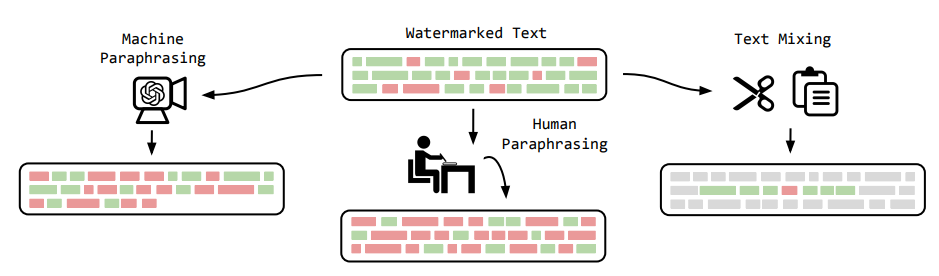
\includegraphics[width=0.5\linewidth]{Images//LR/LR7.png}
    \caption{Watermark robustness under paraphrasing, human edits, and document embedding.}
    \label{fig:LR7}
\end{figure}

%% ============================================================
\section{Research Gaps}
%% ============================================================

Based on the surveyed literature, the following gaps define the open problems addressed by this thesis.

\begin{enumerate}
    \item \textbf{No unified backdoor detection, defense, and watermark preservation.} As summarized in Table~\ref{tab:backdoor_defense}, existing methods address at most two of these three requirements. No single framework simultaneously provides all three capabilities.

    \item \textbf{Detection complexity scales with vocabulary size.} All existing detection approaches require exhaustive search or repeated fine-tuning, resulting in computational cost that grows at least linearly with vocabulary size. Bounded-time detection independent of vocabulary, trigger type, and payload semantics does not exist.

    \item \textbf{Defenses assume known payload types.} Methods such as SANDE and BEEAR construct defense objectives around assumed payload categories, typically hate speech. When payloads are misinformation, sentiment manipulation, or other semantic categories, these assumptions break down and defense effectiveness degrades. No payload-agnostic defense exists.

    \item \textbf{No training-free unlearning for LLMs.} All six surveyed unlearning methods require gradient computation and backpropagation. None can operate in inference-only environments where training-grade GPU resources are unavailable.

    \item \textbf{No single-sample unlearning capability.} Existing methods are designed for batch-level forgetting over curated forget sets. When restricted to a single forget sample, gradient-based methods fail entirely as the signal from one data point is insufficient to drive meaningful parameter updates.

    \item \textbf{No user-initiated unlearning mechanism.} All existing unlearning methods require practitioner access to model internals, training pipelines, and curated datasets. No method enables end users to initiate forgetting through natural language during inference, leaving GDPR and CCPA erasure rights unexercisable in practice.

    \item \textbf{No true test-time knowledge modification.} Existing TTT methods compress context but never remove existing knowledge from model parameters. Persistent weight modification at test time for knowledge removal remains an open problem.
\end{enumerate}